\subsection{Background}

\begin{frame}{Background theories}
    \begin{itemize}
        \item Collaborative learning
        \item Concept mapping to support collaboration
        \item Kit-Build concept mapping approach
    \end{itemize}
\end{frame}

\begin{frame}{Why collaborative learning is important?}

    \begin{figure}[tb]
        \begin{center}
            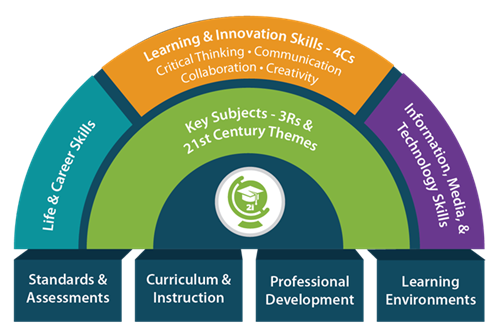
\includegraphics[width=70mm]{images/p21centuryskills.png}
        \end{center}
        \caption{Partnership for 21st century learning. Source: https://www.battelleforkids.org/networks/p21}
        \label{intro::p21}
    \end{figure}
\end{frame}

\begin{frame}{Why collaborative learning is important?}

    \begin{itemize}
        \item<1->  Collaboration is one of the \textcolor{blue}{four-essential skills} in 21st century skills
        \item<1->  The advancement of technology and rapidly changing environment require 
        collaborative works of multidisciplinary experts to solve complex problems effectively
        \item<2->  \textcolor{purple}{However}, collaboration \textcolor{blue}{does not merely happen} just because individuals are co-present 
        \item<2->  It is indeed necessary to practice collaboration in the classroom
    \end{itemize}
\end{frame}

\begin{frame}{Designing learning activities to encourage collaboration}
    \begin{itemize}
        \item<1-> Students' \textcolor{blue}{interactions} play a fundamental role in collaborative learning 
        \cite{Baines2009ImprovingStudy,Webb2009TheClassroom}
        \item<1-> Various instructional strategies are employed to encourage learners to collaborate 
        (i.e. scripts, scenarios, representational tools).
        \item<2> An external representation tool (e.g. concept map) \textcolor{blue}{assists the learner} in articulating and \textcolor{blue}{maintaining shared focus} during discourse \cite{Fischer2002FosteringTools,Suthers2006TechnologyCSCL,vanBoxtel2002CollaborativeDiscourse}.
        %\item<2-> \textcolor{purple}{During collaboration individual learners need to make a continuous effort 
        %to construct and maintain group-shared knowledge \cite{Roschelle1995TheSolving}}. 
        %\item<2-> They may have forgotten prior discussion or feeling difficult to remember 
        %what they have discussed or co-constructed \cite{Jeong2016SevenHelp}.
    \end{itemize}
\end{frame}

\begin{frame}{Applying concept map for collaboration}

    % add concept map figures
    \begin{figure}[tb]
        \begin{center}
            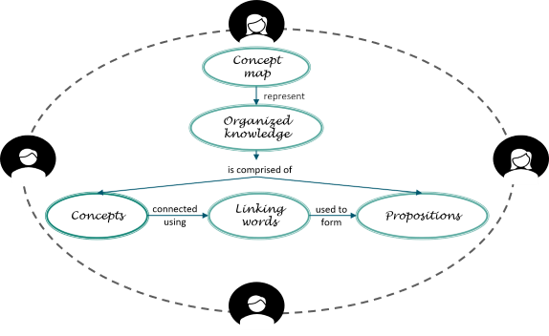
\includegraphics[width=70mm]{images/ccm.png}
        \end{center}
        %\caption{}
        \label{intro::ccm}
    \end{figure}
    
    \begin{itemize}
        \item A concept map has been widely used as a representational tool to \textcolor{blue}{facilitate group discussion}, as well as to \textcolor{teal}{communicate complex ideas} \cite{Fischer2002FosteringTools,Gracia-Moreno2017CollaborativeWorkspaces,Suthers2006TechnologyCSCL,vanBoxtel2000CollaborativeKnowledge}
    \end{itemize}
\end{frame}   

\begin{frame}{Collaborative concept mapping}  
    \begin{itemize}
        % \item<+-> An external representation tool \textcolor{blue}{assist the learner} in articulating and \textcolor{blue}{maintaining shared focus} during discourse \cite{Fischer2002FosteringTools,Suthers2006TechnologyCSCL,vanBoxtel2002CollaborativeDiscourse}
        % \item<+-> A concept map is a graphical tool for organizing and representing knowledge which consists of concepts and relationships among  concepts to facilitate meaningful learning \cite{novak1984learning}.
        %\item<1-2> A concept map has been widely used as a representational tool to \textcolor{blue}{facilitate group discussion}, as well as to \textcolor{teal}{communicate complex ideas} \cite{Fischer2002FosteringTools,Gracia-Moreno2017CollaborativeWorkspaces,Suthers2006TechnologyCSCL,vanBoxtel2000CollaborativeKnowledge}

        \item<1-2> Previous studies posited that collaborative concept mapping has a positive effect on both \textcolor{teal}{students’ attitudes and learning achievements} \cite{Basque2006CollaborativeTrends,Czerniak1998TheScience}.
        
        \item<2-3> However, conflicting evidence has also been found, indicating that students spend a \textcolor{purple}{considerable amount of time} focusing on task collaboration, procedure and team coordination, \underline{rather than} on \textcolor{purple}{discussions about the concepts or relationships involved \cite{chiu2003exploring}}. 
        
        \item<3> Others have also found that students encountered difficulties in \textcolor{purple}{sharing developed ideas and integrating} them into public knowledge \cite{Gracia-Moreno2017CollaborativeWorkspaces,vanBoxtel2000CollaborativeKnowledge} $\longrightarrow$ some \textcolor{purple}{inaccurate ideas are never challenged} and can become ingrained \cite{roth1992social}.
    \end{itemize}
\end{frame}

\begin{frame}{}
    \begin{itemize}
        \item <1-2> It is necessary to design learning activities during collaborative concept map that may \textcolor{teal}{encourage more productive discussion}, as well as, \textcolor{teal}{promote students to share their ideas freely}\\
        \item <2> \emph{Therefore}, we utilize the \textcolor{blue}{Reciprocal Kit-Build (RKB)} before collaborative concept mapping. 
        \item <3>  RKB is an extended version of \textcolor{blue}{Kit-Build (KB)} concept mapping activity to support pair discussion \cite{Wunnasri2018ReciprocalCollaboration,Wunnasri2018ReciprocalUnderstanding}.
    \end{itemize}
    
\end{frame}

\begin{frame}{Kit-Build (KB) concept mapping approach \cite{Hirashima2015}}

    % add concept map figures
    \begin{figure}[tb]
        \begin{center}
            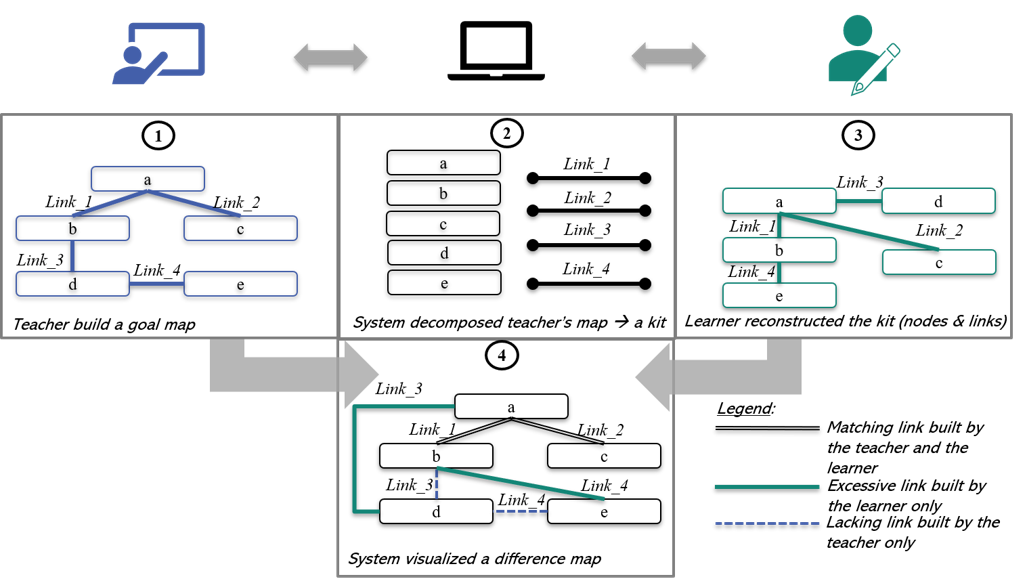
\includegraphics[width=90mm]{images/kb_flow.png}
        \end{center}
        \caption{The KB is a \textcolor{blue}{re-constructional closed-ended approach} to concept mapping
        in which students construct a map based on predefined nodes and
        links extracted from an expert's map \cite{Hirashima2015,Hirashima2019ReconstructionalReconstruction}}
        \label{intro::kbmap}
    \end{figure}
\end{frame}

\begin{frame}{KB concept map for facilitating teacher-student interaction}
    \begin{figure}[tb]
        \begin{center}
            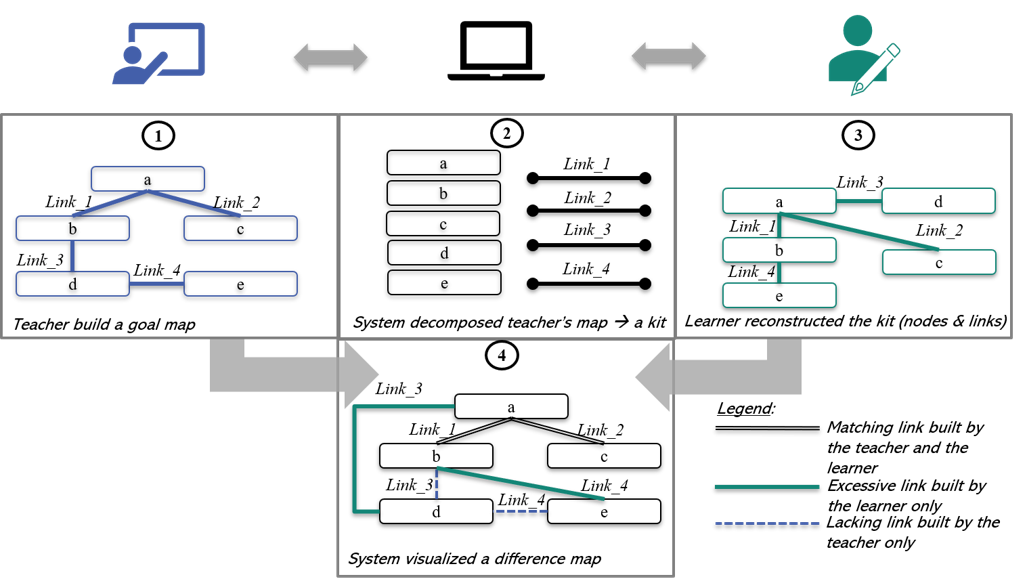
\includegraphics[width=70mm]{images/kb_flow.png}
        \end{center}
    \end{figure}
    
    \begin{itemize}
        \item The KB approach enables teacher to \textcolor{blue}{confirm students' understanding}
        of the information delivered by him/her. 
    \end{itemize}
\end{frame}

\begin{frame}{KB concept map for facilitating teacher-student interaction}
    \begin{figure}[tb]
        \begin{center}
            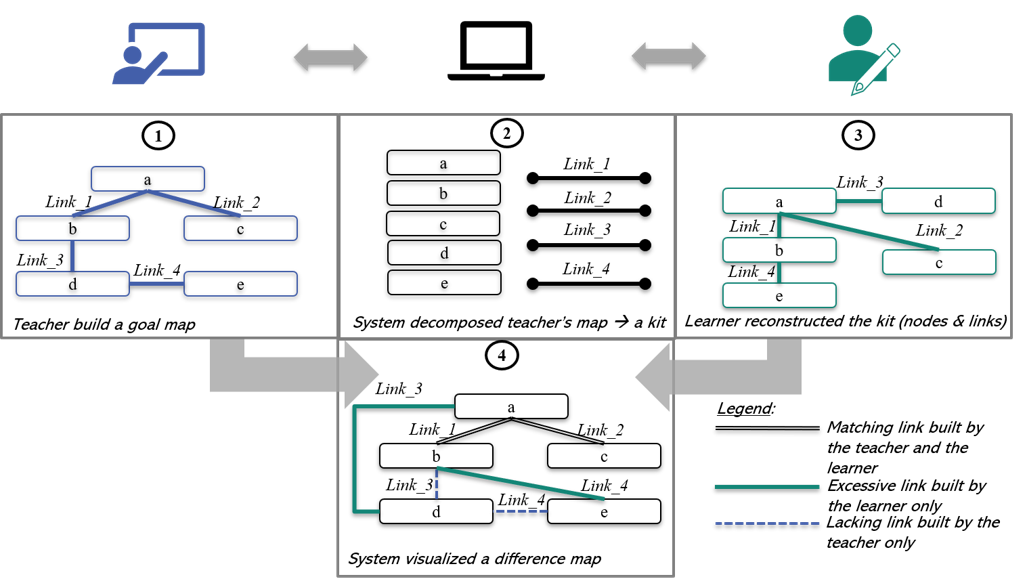
\includegraphics[width=70mm]{images/kb_flow.png}
        \end{center}
    \end{figure}
    
    \begin{itemize}
        \item Moreover, \textcolor{blue}{re-construction} activity provides means to \textcolor{teal}{externalize 
        one's understanding} on the perspective of other.
    \end{itemize}
\end{frame}

% \begin{frame}{KB concept map for facilitating teacher-student interaction}
%    \begin{figure}[tb]
%       \begin{center}
%            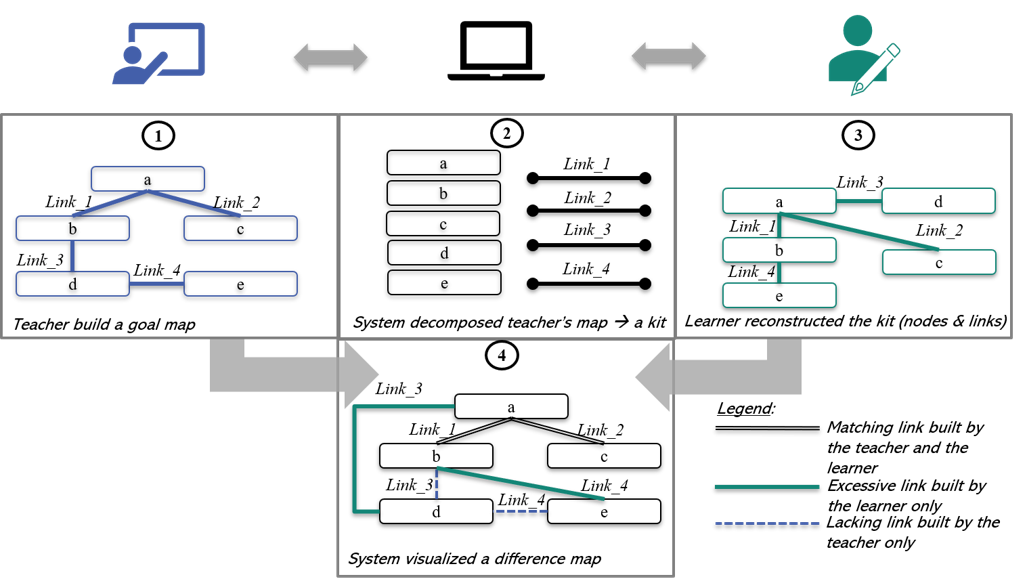
\includegraphics[width=70mm]{images/kb_flow.png}
%        \end{center}
%    \end{figure}
    
%    \begin{itemize}
%        \item Applying KB map approach for peer-to-peer collaboration  $\longrightarrow$ allow students to \textcolor{teal}{communicate empathic understanding}
        
%    \end{itemize}
%\end{frame}

%\begin{frame}{Empathetic collaboration with KB approach}
%    \begin{itemize}
%        \item <+-> Effective \textcolor{blue}{collaboration} is fueled by \textcolor{teal}{empathy} 
%        \item  <+-> To come up with truly  innovative solutions requires new ideas (\textcolor{blue}{creativity}). 
%        \item  <+-> To bring new ideas 
%        to light requires seeking a diversity of perspectives (\textcolor{blue}{critical thinking})
%        and creating a welcoming space for people to share 
%        their ideas without fear of judgment (\textcolor{blue}{communication}).
%    \end{itemize}
%\end{frame}

\begin{frame}{Applying KB concept map for collaboration}
\href{run:/path/nameofvideo.mp4}{\underline{Click for video}}
\end{frame}

\begin{frame}{Differences between KB and RKB}
    \begin{figure}[tb]
        \begin{center}
            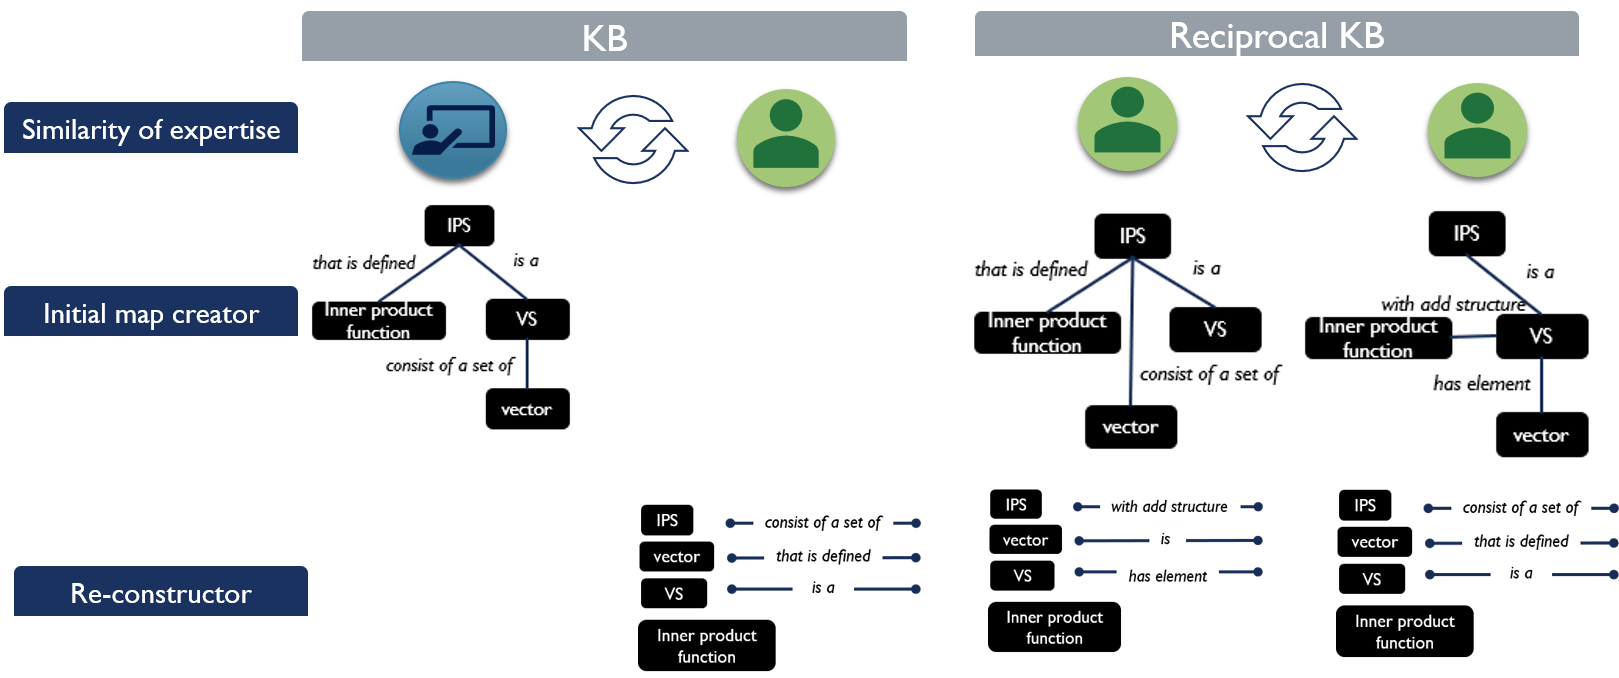
\includegraphics[width=110mm]{images/kb_rkb.pdf}
        \end{center}
        %\caption{Differences between KB and RKB}
        \label{intro::kb_rkb}
    \end{figure}
\end{frame}

\begin{frame}{The roles of reconstruction during RKB}
    \begin{figure}[tb]
        \begin{center}
            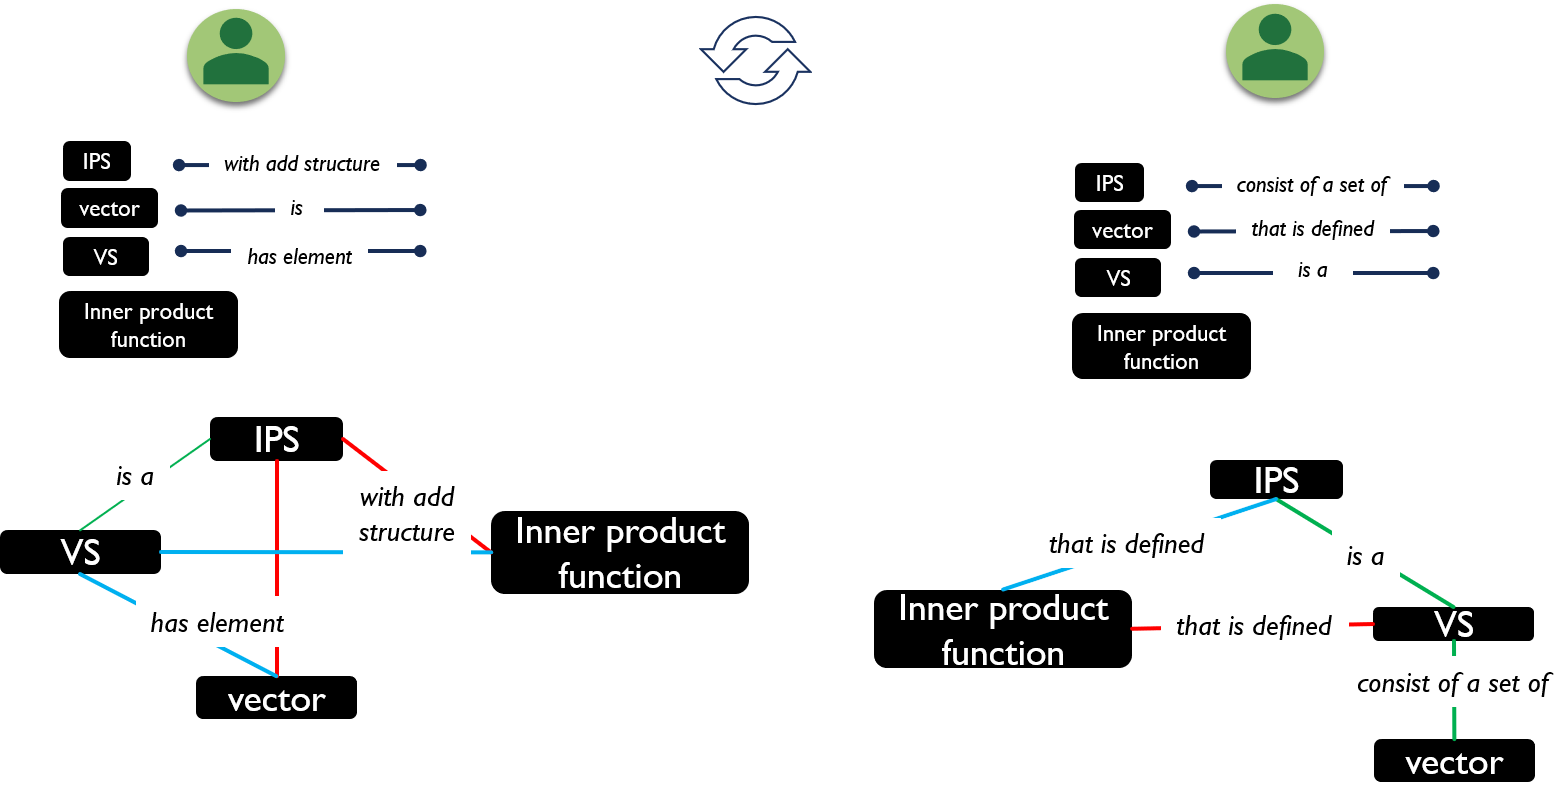
\includegraphics[width=80mm]{images/reconstruction_rkb.png}
        \end{center}
        %\caption{Differences between KB and RKB}
        %\label{intro::kb_rkb}
    \end{figure}
    
    The reconstruction activity triggers students to:
    \begin{itemize}
        \item <2->\textcolor{teal}{communicate empathic understanding}
        \begin{itemize}
            \item <3>\emph{the ability to sense what another individual is thinking or feeling \cite{barak1987increasing}}
        \end{itemize}
        \item <4->\textcolor{teal}{discuss on conflicting ideas}
        
    \end{itemize}
\end{frame}

\begin{frame}{Collaborative concept mapping: existing problems \& potential solutions}  
    
    \begin{columns}
        { \small \begin{column}{0.48\textwidth}
            \begin{itemize}
                \item <1->A \textcolor{purple}{considerable amount of time} focusing on task collaboration, procedure and team coordination \cite{chiu2003exploring}. 
                
                
                \item <1->Difficulties in \textcolor{purple}{sharing developed ideas and integrating} them into public knowledge \cite{Gracia-Moreno2017CollaborativeWorkspaces,vanBoxtel2000CollaborativeKnowledge}.
            \end{itemize}
        \end{column}
    
        \begin{column}{0.48\textwidth}
            \begin{itemize}
                \item <2>RKB provide a \textcolor{blue}{space} for students to \textcolor{teal}{reflect} on individual ideas and \textcolor{teal}{review} their partner's representation
                
                \item <2>Reconstruction activity promote \textcolor{teal}{empathic understanding} and \textcolor{teal}{discussion on conflicting ideas}  
            \end{itemize}
        \end{column}
        }
    \end{columns}
    
\end{frame}

\subsection{Challenges}

\begin{frame}{Initial researches on RKB}
    \begin{itemize}
        \item <1-3> Initial studies showed that the RKB approach \textcolor{blue}{promoted productive
        discussion} between partners (more exploratory talk)
        \cite{Wunnasri2018ReciprocalUnderstanding}. 
        \item <2-3>The RKB map also \textcolor{blue}{encouraged the pair of partners to understand each other} based on the similarity of the individual post-collaboration map
        \cite{Wunnasri2018ReciprocalCollaboration}. 
        \item <3-> $\longrightarrow$ the RKB can be used to \textcolor{teal}{share understanding as preparation for
        collaboration}. 
        \item <4->However, \textcolor{purple}{they have not evaluated the effect of applying
        this approach to build collaborative products}, so far. 
    \end{itemize}
\end{frame}

\begin{frame}{Remaining problems}
    \begin{enumerate}
        \item <1>\textcolor{blue}{Collaborative product evaluation\\} 
        {\small \textcolor{purple}{After following RKB activities, 
        whether or not students are able to achieve high-quality group solutions?}}
        
        \item <2>\textcolor{blue}{Exploring students' perceptions toward the activity\\} 
        {\small \textcolor{purple}{How is the perceptions of the students while following the learning activities?} An evaluation regarding students' acceptance is as important as the learning product itself.}
        \end{enumerate}
  \end{frame}    
\begin{frame}{Remaining problems (cont'd)}
    \begin{enumerate}\setcounter{enumi}{2}
        \item <1> \textcolor{blue}{Analyzing the effect of different group formation on collaboration\\}
        {\small \textcolor{purple}{How different group formation based on their similarity of knowledge may influence collaborative learning effectiveness?} This investigation is needed to unveil the role of RKB for collaboration \& to determine the appropriate group setting} 
        \item <2> \textcolor{blue}{Predicting group outcomes based on individual maps\\}
        {\small \textcolor{purple}{How to foresee students' learning achievements as a group based on the maps created during individual phases (i.e. the initial and re-constructional maps)}? Identifying the relationship between the individual and group products is essential since there is interdependence between these two.} 
    \end{enumerate}
\end{frame}


\subsection{Research objectives}
\begin{frame}{Research objectives}
    Based on the challenges mentioned above, we define the main purposes of this study are as follow: 
    \begin{enumerate}[A]
        \item <1-> {\color<1-2>{blue}to identify the effectiveness of the RKB approach for collaborative concept mapping in a practical classroom};
        \begin{enumerate}
            \item <2-> Collaborative product evaluation
            \item <2-> Exploring students' perceptions toward the activity
        \end{enumerate}
        
        \item <3-> {\color<3-4>{blue} to investigate how individual differences in prior knowledge has potentially influence collaborative-learning effectiveness and the students' perceptions toward the activities}; 
        \begin{enumerate}[3]
            \item <4-> Analyzing the effect of different group formation on collaboration
        \end{enumerate}
        
        \item <5-> {\color<5-6>{blue} to analyze how similarity of individual knowledge and comprehension  of partner's representation could predict the final collaborative products}.
        \begin{enumerate}[4]
            \item <6->Predicting group outcomes based on individual maps
        \end{enumerate}
    \end{enumerate} 
\end{frame}

\begin{frame}{}
    \begin{figure}[tb]
    \begin{center}
        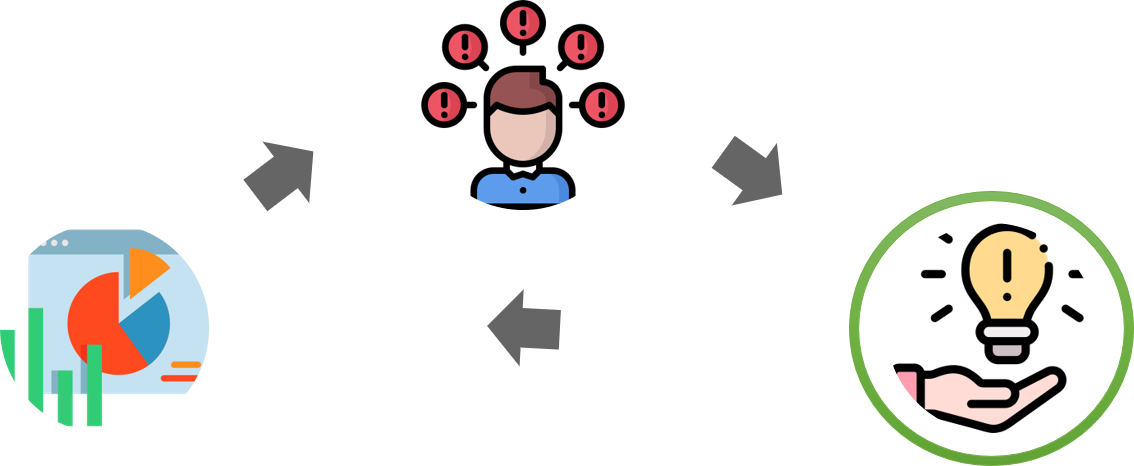
\includegraphics[width=110mm]{images/intro_method.png}
    \end{center}
\end{figure}
\end{frame}

%\subsection{Research objectives}
%\begin{frame}{Research objectives}
%    This study aims to identify the effect of the RKB approach
%    for collaborative learning
%    The purposes of this study are as follow:
%    \begin{itemize}
%        \item <+-> to identify the effect of the RKB approach on collaborative 
%              concept mapping in a practical classroom.
%        \item <+-> to investigate how individual differences in prior knowledge 
%              may influence collaborative-learning effectiveness 
%              (e.g. transfer of knowledge, lost knowledge, group product) 
%              and the students' affective responses toward the activities. 
%        \item <+-> to investigate how individual prior knowledge convergence and comprehension 
%            levels through reconstruction may potentially predict the final 
%            collaborative product. 
%    \end{itemize} 
%\end{frame}